\documentclass{beamer}
\usepackage[utf8]{inputenc}
\usetheme{Warsaw}

\title{Nintendo Entertainment System}
\author{Jonathan Sieber}

\begin{document}
    \maketitle
    \begin{frame}
    \frametitle{}
    \begin{itemize}
        \item{aus Gründen}
    \end{itemize}
    \end{frame}
    
    
    \begin{frame}
        \frametitle{Das Ziel}
        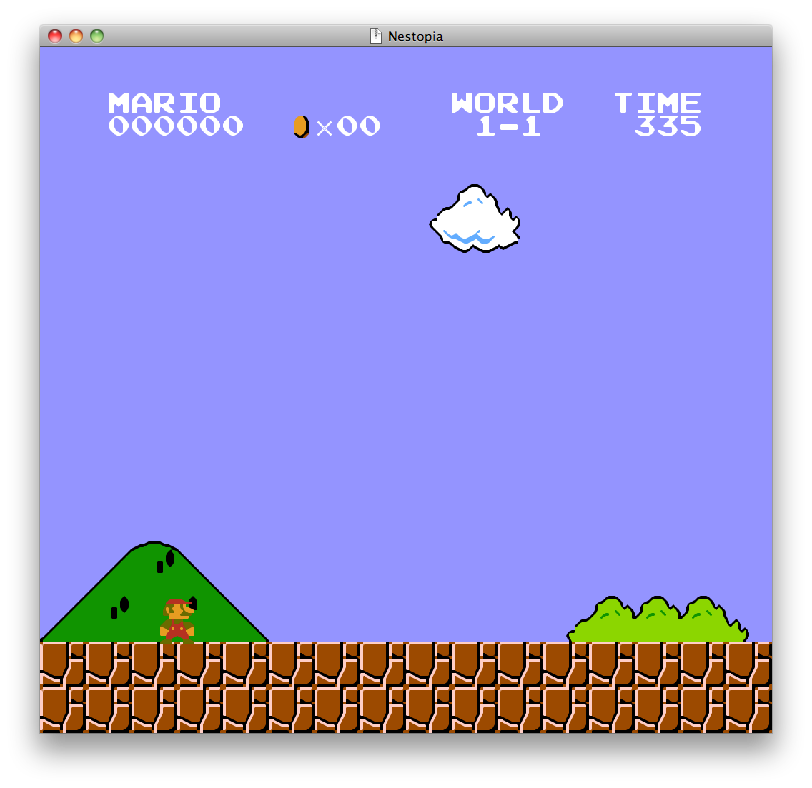
\includegraphics[width=0.8\linewidth]{img/smb.png}
    \end{frame}
    
    \begin{frame}
        \frametitle{Nintendo Entertainment System}
        \begin{itemize}
            \item{1983 als Nintendo Famicom in Japan veröffentlicht}
            \item{Erste erfolgreiche Konsole nach dem Video Game Crash}
            \item{Programm/Grafik-Speicher durch Cartridges leicht erweiterbar}
        \end{itemize}
    \end{frame}
    
    \begin{frame}
        \frametitle{CPU}
        \begin{itemize}
            \item{Custom Chip Ricoh 2A03 @ 1.76 MHz}
            \item{Basiert auf MOS Technology 6502}
            \item{Enthält Soundchip mit 5 Tongeneratoren}
            \item{DMA-Kanal für Sprite-Updates auf PPU}
            \item{Schon 1983 langsam, Innovation auf PPU}
        \end{itemize}
    \end{frame}
    
    \begin{frame}
        \frametitle{CPU}
        \begin{itemize}
            \item{Ricoh RP2C02}
            \item{@5.37 Mhz = NTSC Pixel Clock}
            \item{Gibt direkt analoges NTSC-Signal aus, kein Framebuffer}
            \item{1 Background Layer}
            \item{64 Sprites}
        \end{itemize}
    \end{frame}
    
    \begin{frame}
        \frametitle{Background Layer}
        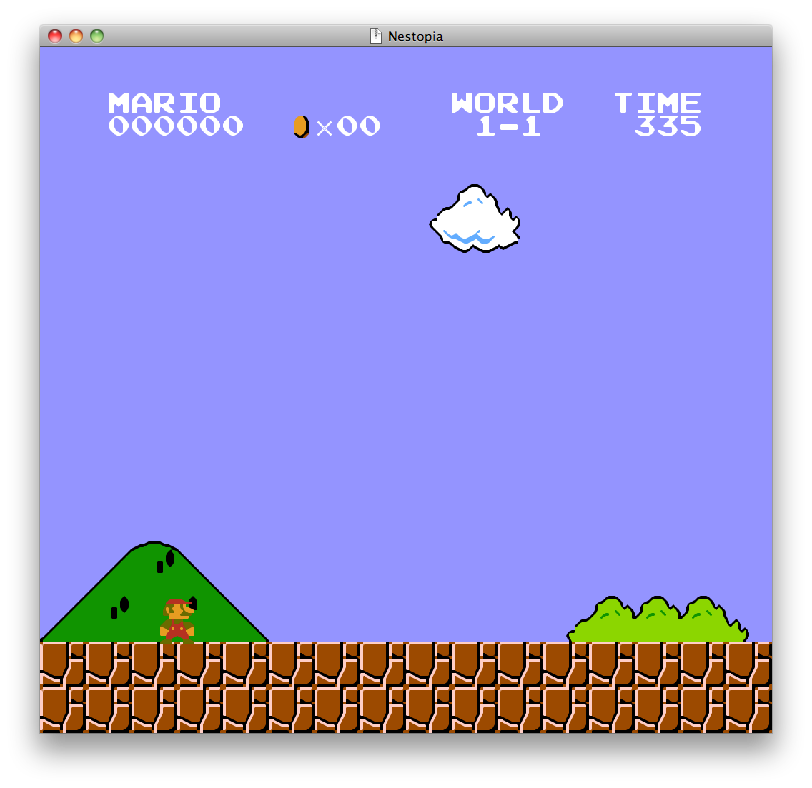
\includegraphics[width=0.8\linewidth]{img/smb_bg.png}
    \end{frame}
    
    
    \begin{frame}
        \frametitle{Sprite Layer}
        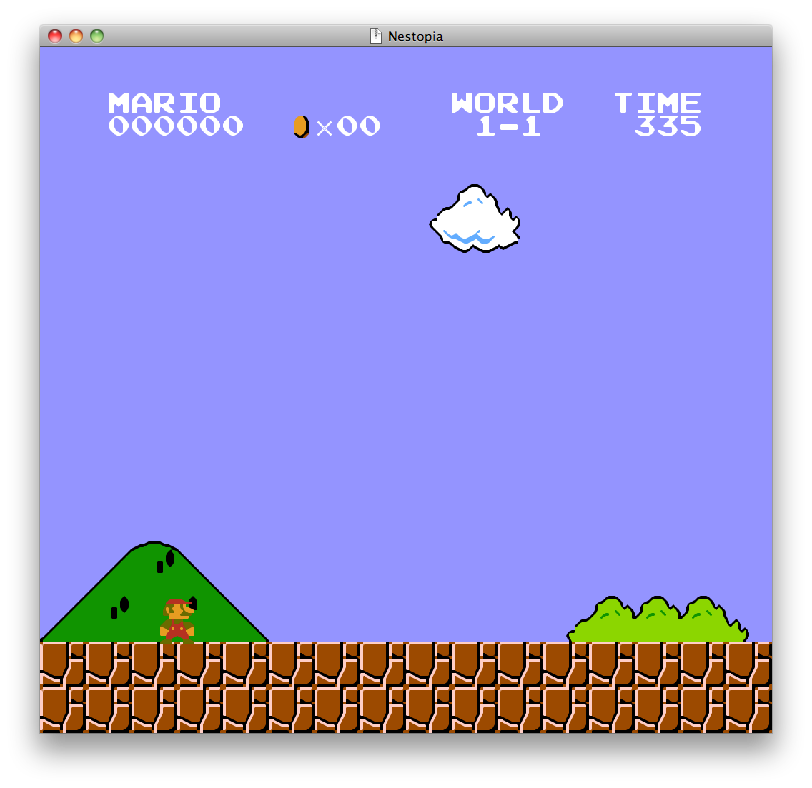
\includegraphics[width=0.8\linewidth]{img/smb_sprite.png}
    \end{frame}
    
    \begin{frame}
        \frametitle{Ausgangslage}
%            \begin{column}{5cm}
            \begin{block}{5cm}
                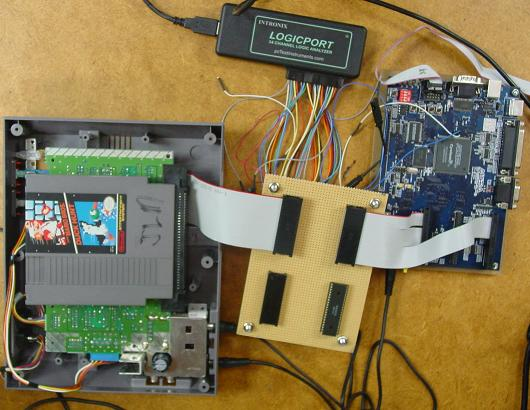
\includegraphics{img/danleach.jpg}
            \end{block}
%            \begin{column}
                \begin{itemize}
                    \item{Master Thesis von Dan Leach (Bradley University)}
                    \item{Ersetzt die CPU aus Original-Hardware}
                    \item{Basiert selbst auf 6502-Implementierung von fpgaarcade.com}
                    \item{Konnte mit geringen Anpassungen verwendet werden}
                    \item{Noch ohne Soundgenerator}
                \end{itemize}
%            \end{column}
%        \end{columns}
    \end{frame}
    
    
    \begin{frame}
        \frametitle{Bereits geschafft}
        \begin{itemize}
            \item{HDMI Ausgabe}
            \item{System mit Super Mario ROM}
            \item{PPU Background Layer}
        \end{itemize}
    \end{frame}
    
    \begin{frame}
        \frametitle{Noch zu tun}
        \begin{itemize}
            \item{PPU Scrolling, Sprites und weitere Details}
            \item{Controller Input}
            \item{Memory Mapper für größere Spiele}
        \end{itemize}
    \end{frame}
    
\end{document}
